\documentclass{beamer}

\setbeameroption{hide notes} % Only slides
% \setbeameroption{show only notes} % Only notes
% \setbeameroption{show notes on second screen=right} % Both

% \usepackage{../AssertionEvidence.sty}
\usetheme{Madrid}
\usepackage{hyperref}
\usepackage{graphicx}
\usepackage{tikz}
\usepackage[style=verbose,backend=biber]{biblatex}

\defbeamertemplate*{title page}{customized}[1][]{
\begin{center}
  \usebeamerfont{title}\inserttitle\par
  \usebeamerfont{subtitle}\usebeamercolor[fg]{subtitle}\insertsubtitle\par
  \bigskip
  \usebeamerfont{author}\insertauthor\par
  \usebeamerfont{institute}\insertinstitute\par
  \usebeamerfont{date}\insertdate\par
  \usebeamercolor[fg]{titlegraphic}\inserttitlegraphic  
\end{center}  
}

\graphicspath{ {../imgs/} }

% Add above to the style

\title{Introduction to Artificial Intelligence}
\subtitle{The foundation and history of Artificial Intelligence and its Applications}
\author[RMS]{Rojesh Man Shikhrakar}

\begin{document}
\maketitle

\begin{frame}
  \frametitle{Syllabus: Unit 2: Problem Solving Methods [12 Hrs]}

  \begin{itemize}
    \item 2.1 Definition of a Problem, Problem as a state space representation, Problem formulation, Well-defined problems, Constraint satisfaction problem, Water jug problem-Queen problem, Cryptarithmetic problem, Graph coloring problem
    \item 2.2 Problem solving by searching, types of searching, measuring problem solving performance, General State Space Search
    \item 2.3 Uninformed: Breadth-First Search, Depth-First Search, Depth-Limited Search, Iterative Deepening depth first Search, Bidirectional Search, using uninformed search techniques for solving N-Queens Problem, Puzzle problem etc.
    \item 2.4 Informed search: Greedy Best-First Search, A* Search, Optimality of A*, Local search: Hill Climbing, Simulated Annealing, 
    \item 2.5 Game Playing, Optimal Decisions in Games, Alpha — Beta Pruning, Minimax Algorithm, Tic-Tac —Toe Problem, Stochastic Games
  \end{itemize}
\end{frame}

\begin{frame}
  \frametitle{Search or planning Agents are agents that plan ahead}
  \framesubtitle{Evaluates how the model evolves based on the future action sequence}
  \begin{columns}
    \column{0.4\textwidth}
    \begin{center}
      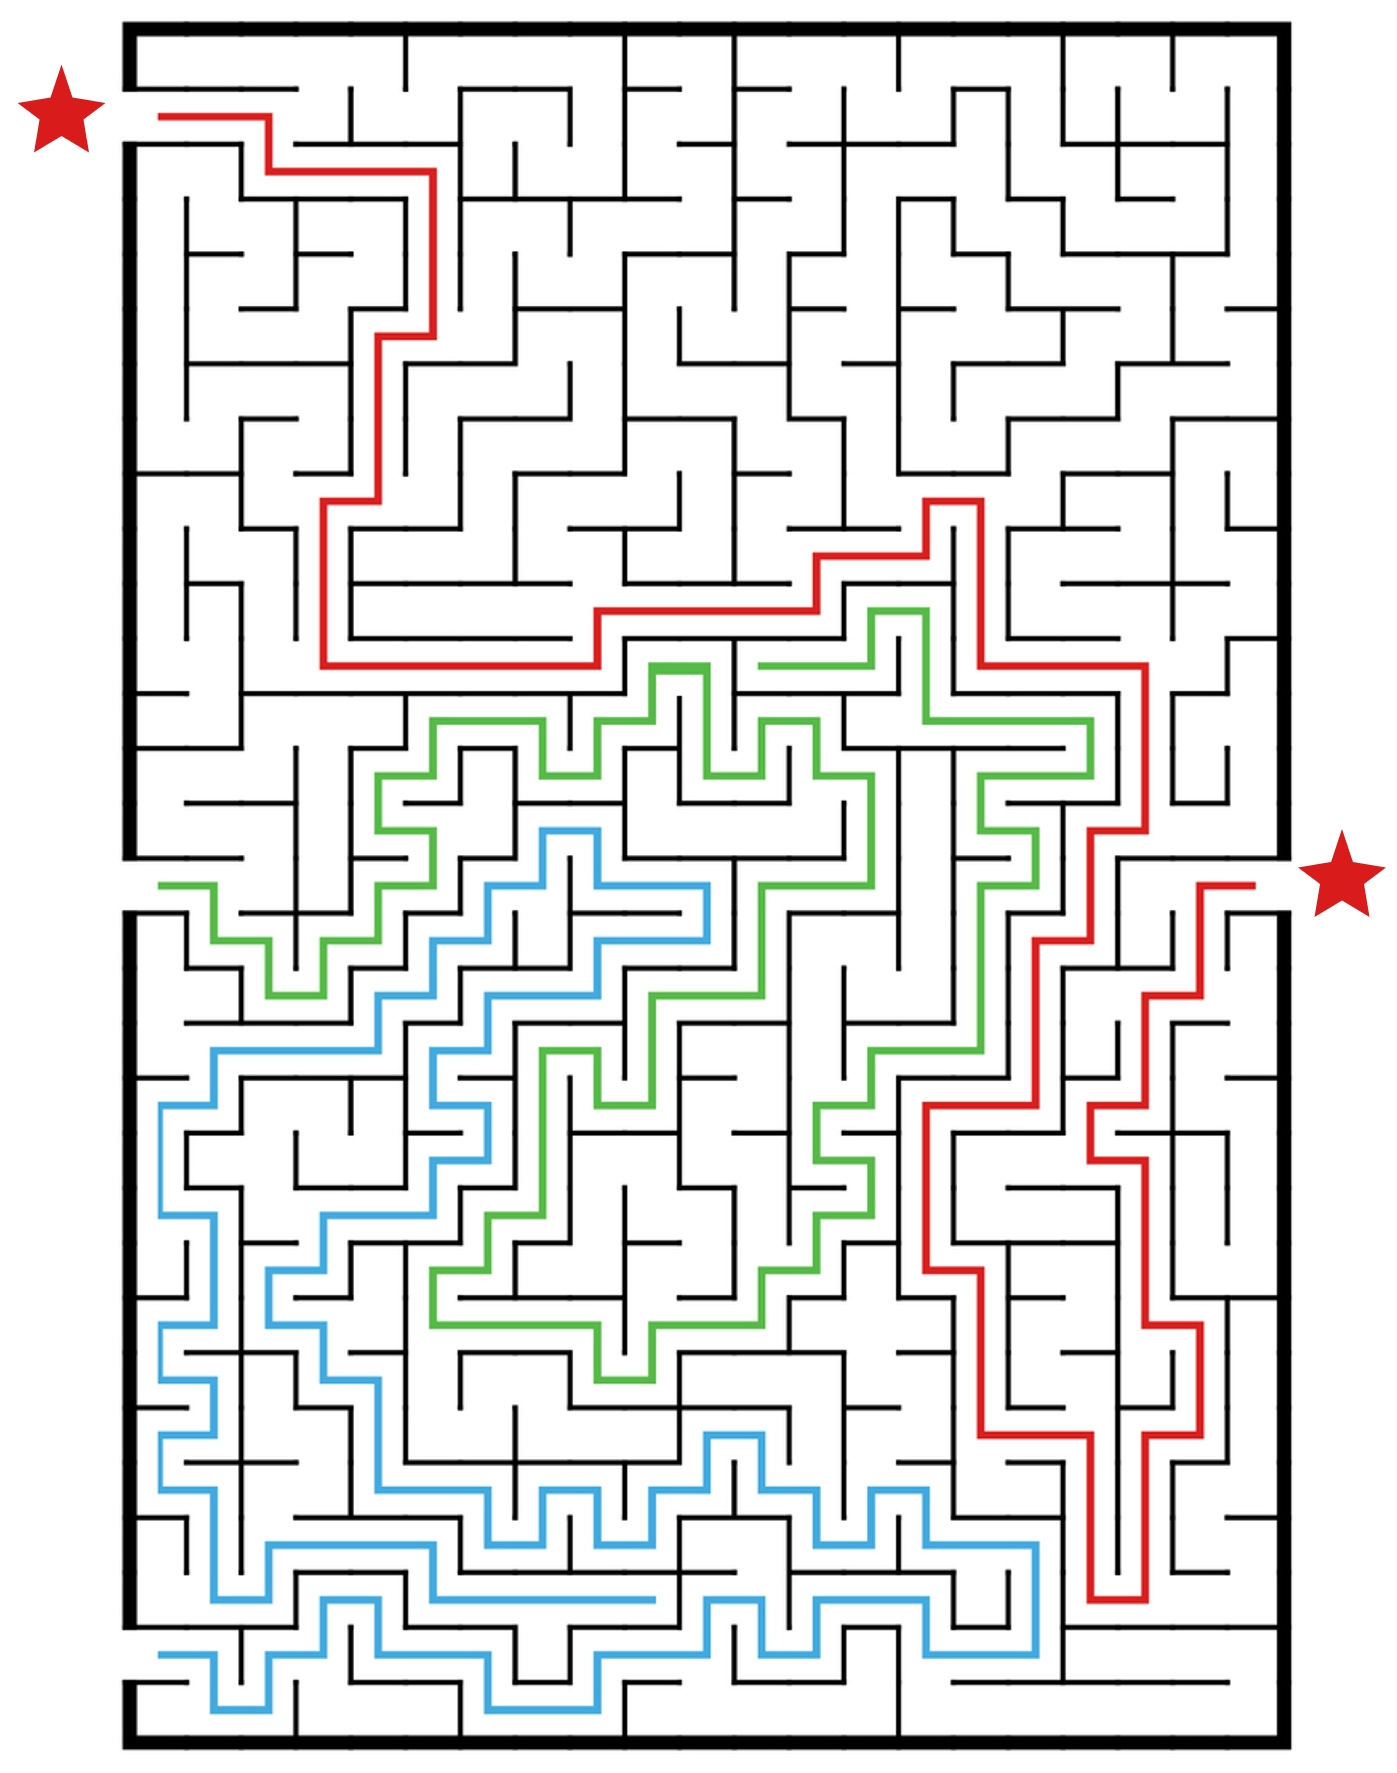
\includegraphics[width=\textwidth]{MazeMultiplePathways.jpg}
    \end{center}
    \column{0.6\textwidth}
      \begin{itemize}
        \item Model how the world evolves in response to action
        \item Agent evaluates future action sequences
        \item Usually have a definite goal
        \item Optimality is to achieve least cost path
      \end{itemize}
  \end{columns}

\end{frame}

\begin{frame}
  \frametitle{Problem Formulation: }
  A search Problem consists of :
  \begin{itemize}
    \item A state space $S$
    \item An initial state $s_0$
    \item Actions $A(s)$ in each state
    \item Transition model Result(s,a)
    \item Goal Test G(s)
    \item Action cost c(s,a,s')
  \end{itemize}
  
  Solution of search problem is an action sequence that reaches a goal state. 
  
  An optimal solution has least cost among all solutions.

\end{frame}



\end{document}